\section{Methodology}
\label{sec:methodology}
\subsection{Problem formulation}
\label{sec:prob-formulation}
Given an input surveillance video containing $N$ frames, we want to produce a binary time series of same length $N$ such that at each index $i$, we have the label $y_i$ of the corresponding frame $f_i$ . The human trespassing label is assigned to positive class (1) while the ``other activity'' label is assigned to negative class (0). Since each prediction depends only on the corresponding frame $f_i$, our problem boils down to determining a function $D$ with parameter $\theta$ such that:
$$ D(f_i;\theta) = \hat{y}_i $$
The aim is to find a $\theta^*$ such that $D(f_i;\theta^*) \rightarrow y_i$ where $y_i$ is the ground truth label corresponding to $f_i$. The ground truth label has the following definition: 
$$y=
\begin{cases}
1,  &\qquad \textrm{if } f_i \textrm{ contains trespassing activity} \\ 
0, 	&\qquad \textrm{otherwise}
\end{cases}
$$
We define trespassing activity as the presence of at  least one person in the frame. 

%\subsection{Proposed framework}
\subsection{ARTS framework}
\label{sec:proposed-framework}
%In order to tackle this problem, we propose a two-stage trespassing detection model. 
%This model is in accordance with our approach in Section \ref{sec:approach}. 
Figure \ref{fig:trespassing-detection-framework} shows the outline of our proposed ARTS framework. In the first stage, we decide whether a particular frame has an activity or not. If it turns out that the given frame has no activity, then it is classified as background frame. No further action needs to be taken for this frame. On the other hand, if it shows activity, then the next step (stage 2) is to investigate whether it can be classified as human trespassing activity or not. The rationale for using dual-stage architecture is that the first stage is much faster than the second stage. This allows the first stage to filter out most of the non-activity frames and therefore only prospective frames are processed by stage 2.


Figure \ref{fig:trespassing-detection-pipeline} illustrates the pipeline modeling the ARTS framework.
Input to our pipeline is a video with each frame being processed one by one. Only the frames classified as  ``activity frames" are further processed through stage 2. Output of the ARTS corresponds to a time series as discussed in Section \ref{sec:prob-formulation}. 

Input to the stage 1 is a video frame whereas the output is a binary decision indicating whether it is an activity frame or background frame. The stage 2 not only gets the output of stage 1 as input, but also the corresponding frame. It skips the processing of the frame in case it is of the background type; otherwise, it processes the frame for verification of the human trespassing activity. The output of stage 2 is also a binary decision indicating the human trespassing activity or other activity. Concatenation of the stage 2 output for each input frame produces the output time series. The proposed ARTS framework is extremely flexible in the sense that it allows any pair of algorithms to construct the trespassing detection pipeline given they perform the respective functions of stage 1 and stage 2. Apart from that, the only restriction is that the processing time per frame of stage 1 algorithm should be much less than that of stage 2 algorithm to reap the practical benefit of ARTS. 

\begin{figure}
    \centering
    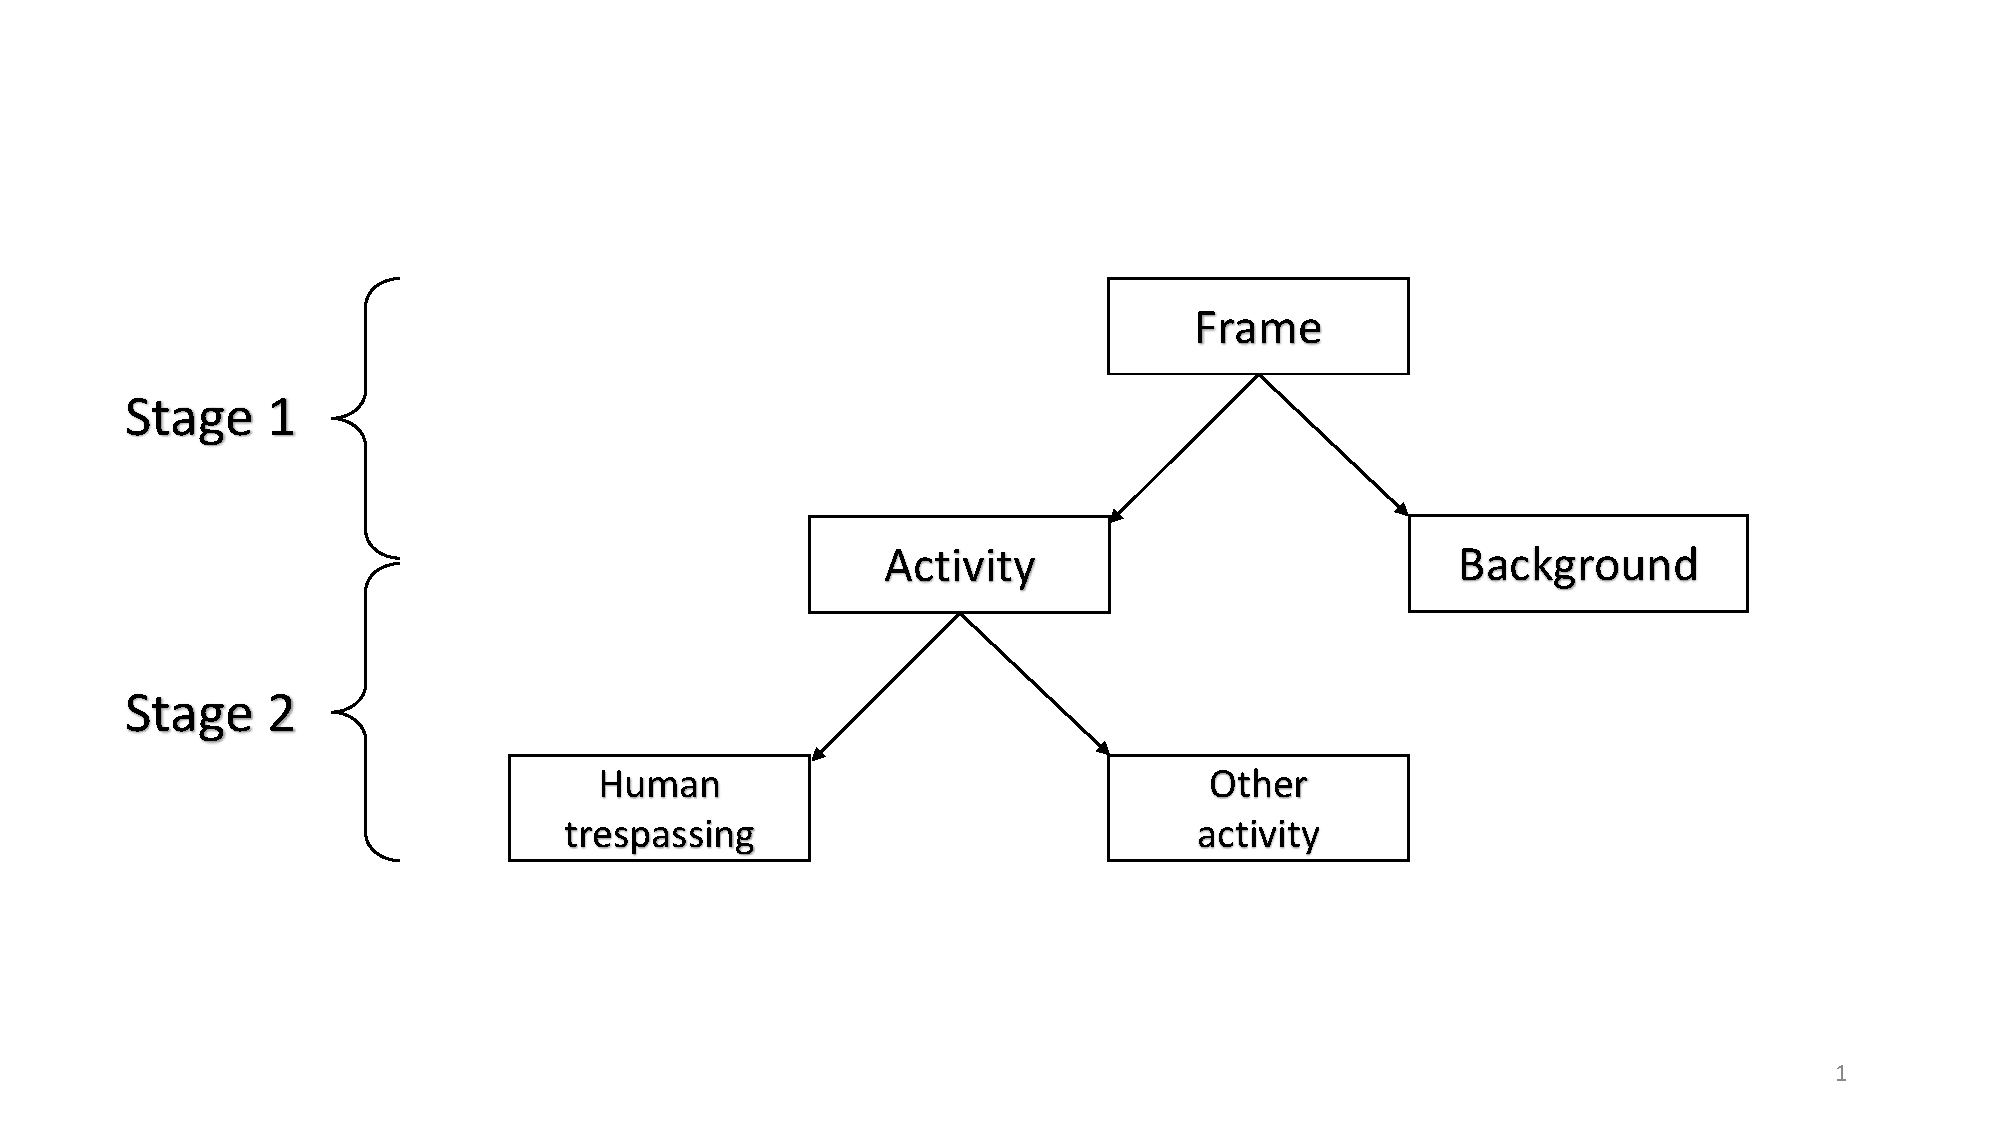
\includegraphics[width=\linewidth,trim={50 110 50 130},clip]{images/trespassing-detection-framework}
    \caption{Trespassing detection framework}
    \label{fig:trespassing-detection-framework}
\end{figure}


\begin{figure}
    \centering
    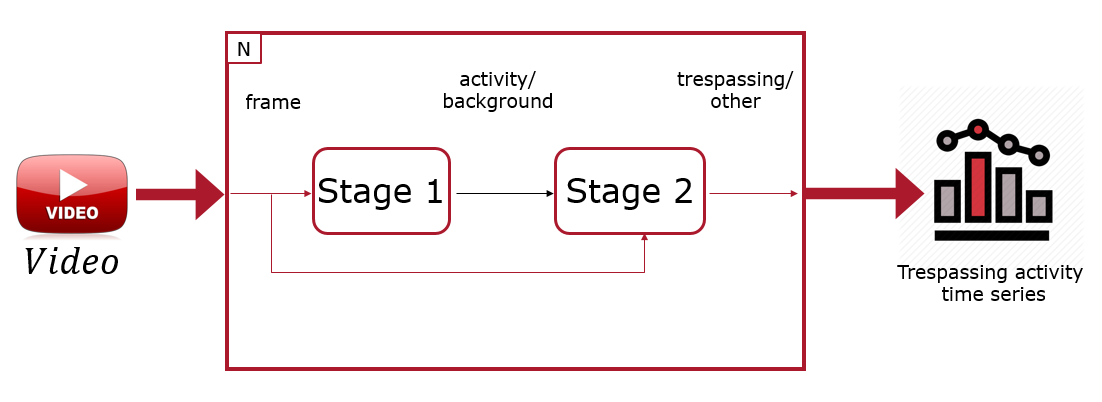
\includegraphics[width=\linewidth,trim={0 110 0 130},clip]{images/trespassing-detection-pipeline}
    \caption{Trespassing detection pipeline}
    \label{fig:trespassing-detection-pipeline}
\end{figure}


\subsection{Stage 1 of the ARTS framework}
\label{sec:stage1}
The goal of this first stage is to filter non-activity frames from the activity frames. Thus, it is modeled as a background subtraction problem. Figure \ref{fig:background-subtraction-model} shows the block diagram of background subtraction method. 
\begin{figure}
    \centering
    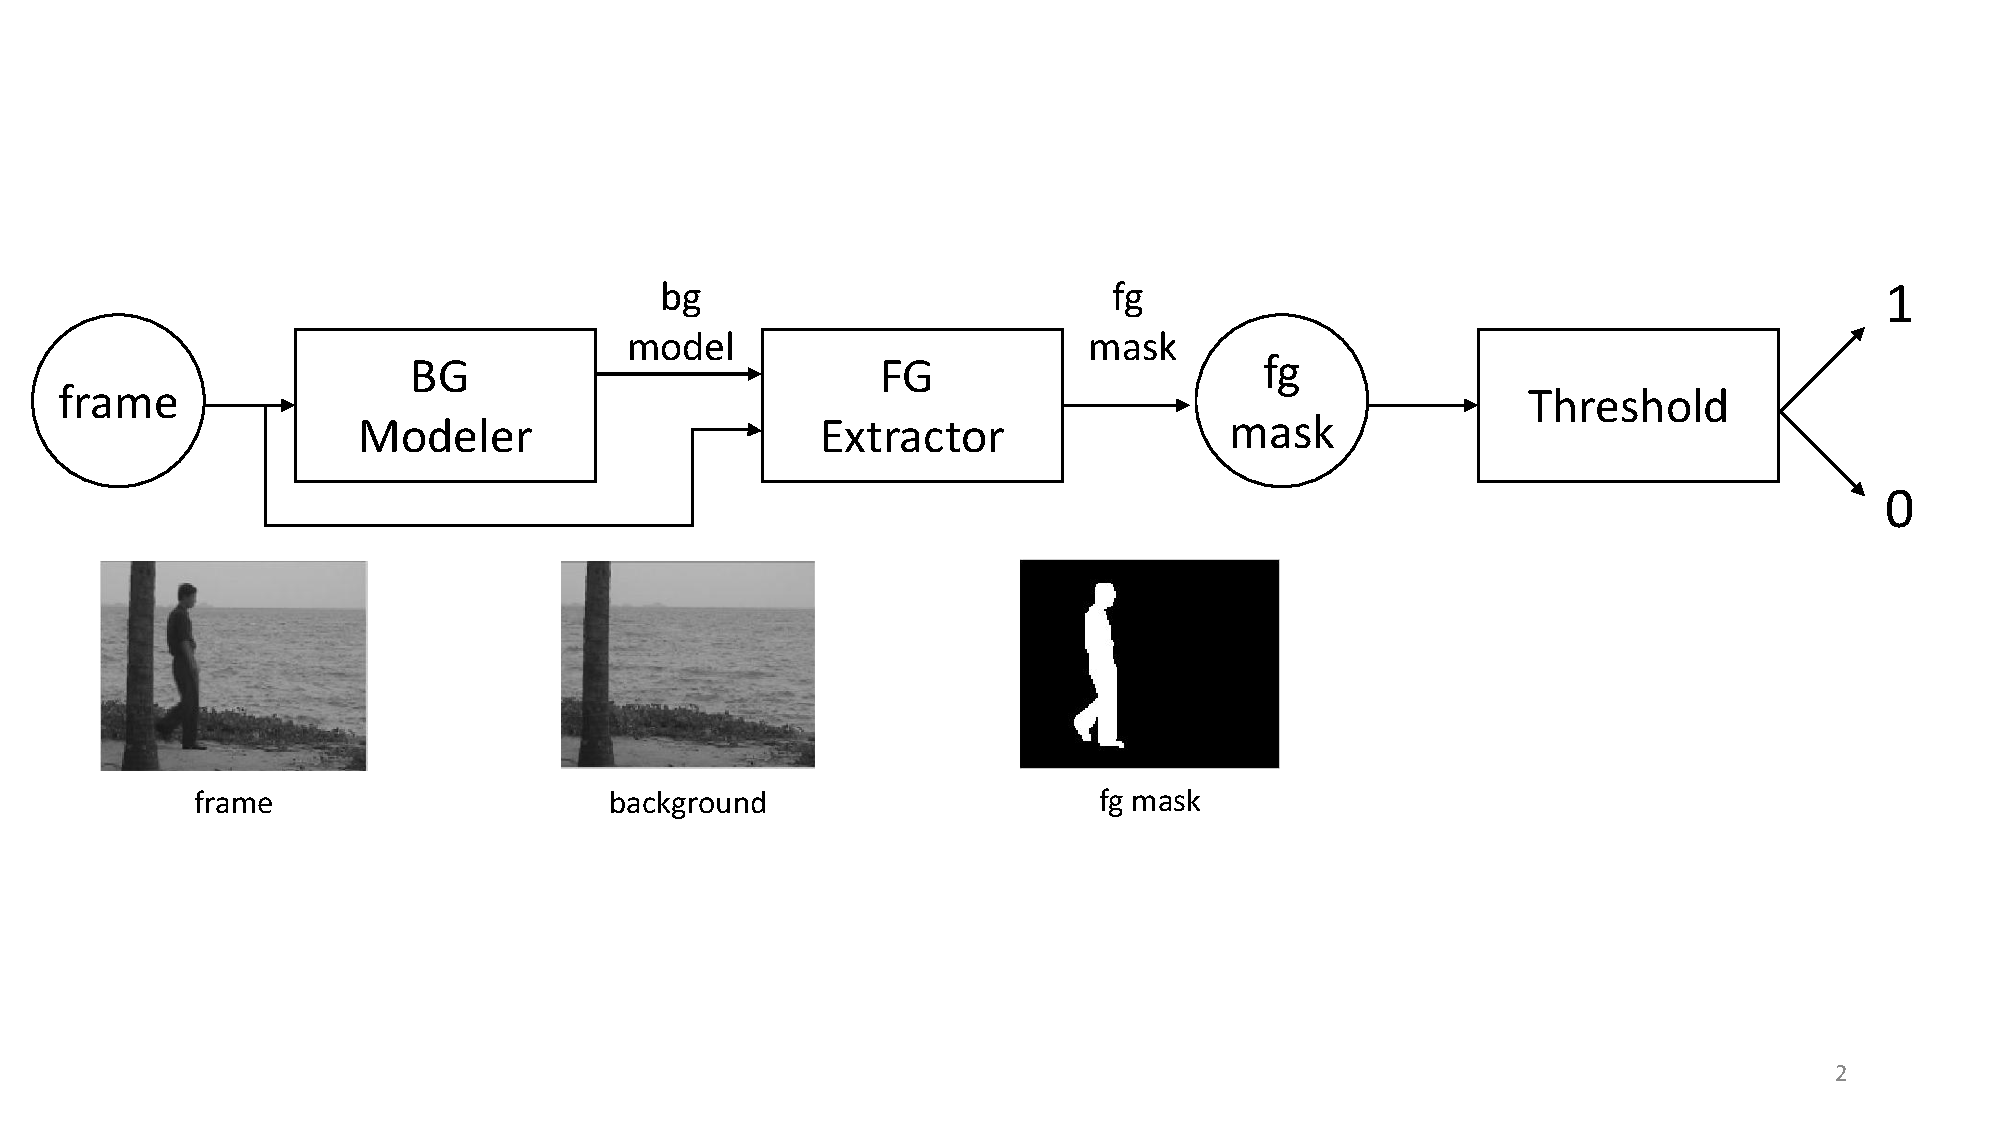
\includegraphics[width=\linewidth,trim={0 130 0 130},clip]{images/background-subtraction-model}
    \caption{Stage 1 - Background subtraction model}
    \label{fig:background-subtraction-model}
\end{figure}

We propose to model the background as mixture of gaussians \cite{stauffer1999adaptive,power2002understanding}. Since, an image usually represents many different surfaces (objects), each surface is expected to give rise to a new gaussian. Thus all pixel values are better represented by a mixture (sum) of gaussians. Notice that this model represents both foreground and background simultaneously. In order to apply this model to the background subtraction problem, we associate each pixel with a particular surface and then associate that surface with either foreground or background. The label of each pixel, namely either foreground or background, is determined by the label of the corresponding surface. 

\subsubsection{Background (BG) modeler}
Each surface (or uniform object) that comes into the camera view is represented by a state $k \in {1,2,3,...,K}$. Some of these states correspond to  background while the remaining ones are considered to be foreground. The process  $\mathbf{k}$ which generates the states is modeled by parameters set $\{w_1, w_2, ..., w_K\}$ where $w_k = P(k)$. Each of these parameters represents  a priori probability of surface $k$ appearing in the image. Further we have, $\sum_{k=1}^K w_k=1$. 

This surface process $\mathbf{k}$ is hidden and is only indirectly observable through the pixel value process $\mathbf{X}$. The pixel value process $\mathbf{X}$ is an observable random variable modeled by a gaussian process for given surface $k$. $\mathbf{X}$ is 1-D in case of gray scale images and 3-D for color images.  If $\theta_k= \{\mu_k, \Sigma_k \}$  represent the associated gaussian process then pixel value process $\mathbf{X}$ given $k$ is: 

$$ f_{\mathbf{X}|k}(X|k,\theta_k)=\frac{1}{\sqrt{(2\pi)^n |\Sigma_k |}}e^{-\frac{1}{2}(X-\mu_k)^T \Sigma_k^{-1} (X-\mu_k)} $$
where $\mu_k$ denotes the mean and $\Sigma_k$ is the covariance matrix of the associated $k^{th}$ gaussian. 

We assume these $k$ events are disjoint so $\mathbf{X}$ can be modelled as the sum of gaussians. 

$$ f_{\mathbf{X}}(X|\Phi)=\sum_{k=1}^K w_k f_{\mathbf{X}|k}(X|k,\theta_k)  $$
where $ \Phi = \{w_1, \mu_1, \Sigma_1,..., w_K, \mu_K, \Sigma_K \}$ 

\subsubsection{Foreground (FG) modeler}
In order to apply the model to our background subtraction problem, the first step is to determine which of the $K$ states is most likely to give rise to current pixel value $\mathbf{X}=X$. The posterior probability $P(k|X,\Phi)$ denotes the likelihood that pixel value $X$ was generated by surface $k$. Using the Bayes's theorem, we have:

$$ P(k|X,\Phi) = \frac{P(k)f_{\mathbf{X}|k}(X|k,\Phi)}{f_\mathbf{X}(X,\Phi)} $$
The k which maximizes the $P(k|X,\Phi) $ is considered to be the surface associated with $X$.

$$ \hat{k}=\operatorname*{argmax}_k P(k|X,\Phi)$$

Once $X$ has been associated with a particular surface $\hat{k}$, it needs to be determined whether $\hat{k}$ is a foreground surface or background. 

The procedure for demarcation starts with ranking K states by $w_k / | \Sigma_k |$ in decreasing order. This ratio is proportional to the height of the weighted distribution $w_k f_{\mathbf{X}|k}(X|k,\theta_k)$. A surface $k$ is considered to be a background if it occurs more frequently (higher $w_k$) and does not vary much (low $|\Sigma_k|$).  To separate the foreground and background surfaces, an overall prior probability $T$ of anything being in the background is used. The first $B$ of the ranked  states whose accumulated probability crosses the threshold $T$ are considered to be background. 
$$ B=\operatorname*{argmin}_b (\sum_{j=1}^b w_{j} > T)$$ 

\subsubsection{Threshold}
The output of the foreground extractor is a binary mask which indicates whether a pixel belongs to the foreground or not. All the foreground pixels in the image can be summed up and their ratio to the total number of pixels in the frame can be compared to a threshold value $\tau$. If the ratio is greater than the threshold, then this frame is regarded as activity frame (1); otherwise it is classified as background frame (0). 


\subsection{Stage 2 of the ARTS framework}
\label{sec:stage2}
The goal of this second stage is to verify human trespassing in the case of activity reported by stage 1. The state-of-the-art deep learning model Faster-RCNN\cite{ref_fasterrcnn} is used to model this stage. Faster-RCNN predicts the label and location of the objects corresponding to the input frame. The given image is labelled with \textit{trespassing activity} if there is at least one person predicted by Faster-RCNN with corresponding confidence score greater than a threshold $\nu$. Figure \ref{fig:faster-rcnn-pipeline} depicts the block diagram of Faster-RCNN with a detailed explanation given below: 


\begin{figure}
    \centering
    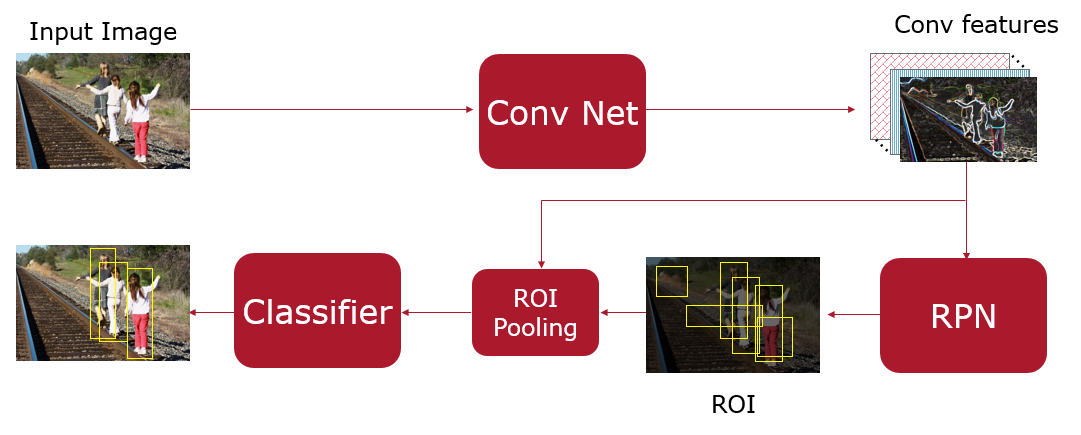
\includegraphics[width=\linewidth,trim={0 80 0 120},clip]{images/faster-rcnn-pipeline}
    \caption{Stage 2 - Faster-RCNN block diagram}
    \label{fig:faster-rcnn-pipeline}
\end{figure}

\vspace{5pt}
\subsubsection{Feature extraction (Conv. Net)}
\label{sec:feature-extraction}
The first step is to extract the convolutional features, also known as feature map, from the input frame. These convolutional features will be used by subsequent sub-stages as input. Due to the paramount importance of features generated by this sub-stage, it is also known as the backbone of Faster-RCNN. It can be modelled using VGG\cite{simonyan2014very} or Resnet\cite{he2016deep}. Here in this work, we adopt the Resnet-50 network with Feature Pyramidal Network (FPN) \cite{lin2017feature} for our experiments. 

\vspace{5pt}
\subsubsection{Region Proposal Network (RPN)}
This sub-stage as the name suggests is responsible for proposing regions (rectangles) potentially containing objects (people, cars, etc). As seen in Figure \ref{fig:faster-rcnn-pipeline}, this sub-stage takes in the feature map and produces a list of proposals for the given image. Each proposal consists of a binary label and the proposed bounding box of the region of interest. The label then indicates whether the proposal corresponds to an object or the background. 
%The proposals thus produced by the network are subjected to non-maximum suppression. This process removes the duplicate proposals and makes subsequent processing more efficient. 

\vspace{5pt}
\textit{a. Anchors of RPN}\\
Anchor act as default region proposals. Their whole idea has been motivated by multi-scale sliding windows \cite{ref_fasterrcnn}. Suppose we use a feature extraction convolutional network such that it converts a $800\times800$ image to $50\times50$ feature map (Figure \ref{fig:anchors}). This means every $(x,y)$ location on the feature map corresponds to a $16\times16$ window on the original image. Similarly, an $8\times8$ window on the feature map corresponds to a $128\times128$ window on original image. This $8\times8$ window on the feature map is known as anchor. Faster-RCNN proposes multi-scale, multi-aspect ratio anchors. A total of 3 scales (8, 16, 32 on the feature map) with 3 aspect ratios ($1:1$, $1:2$, $2:1$) produce 9 anchors on each $(x,y)$ location of the feature map. Since we have $50\times50$ locations, this setting produces 22,500 anchors in total. However, in practice we use far less than that number. All anchors whose regions lie outside the feature map (e.g., anchors near edges), don't participate in training the network. 

\begin{figure}
    \centering
    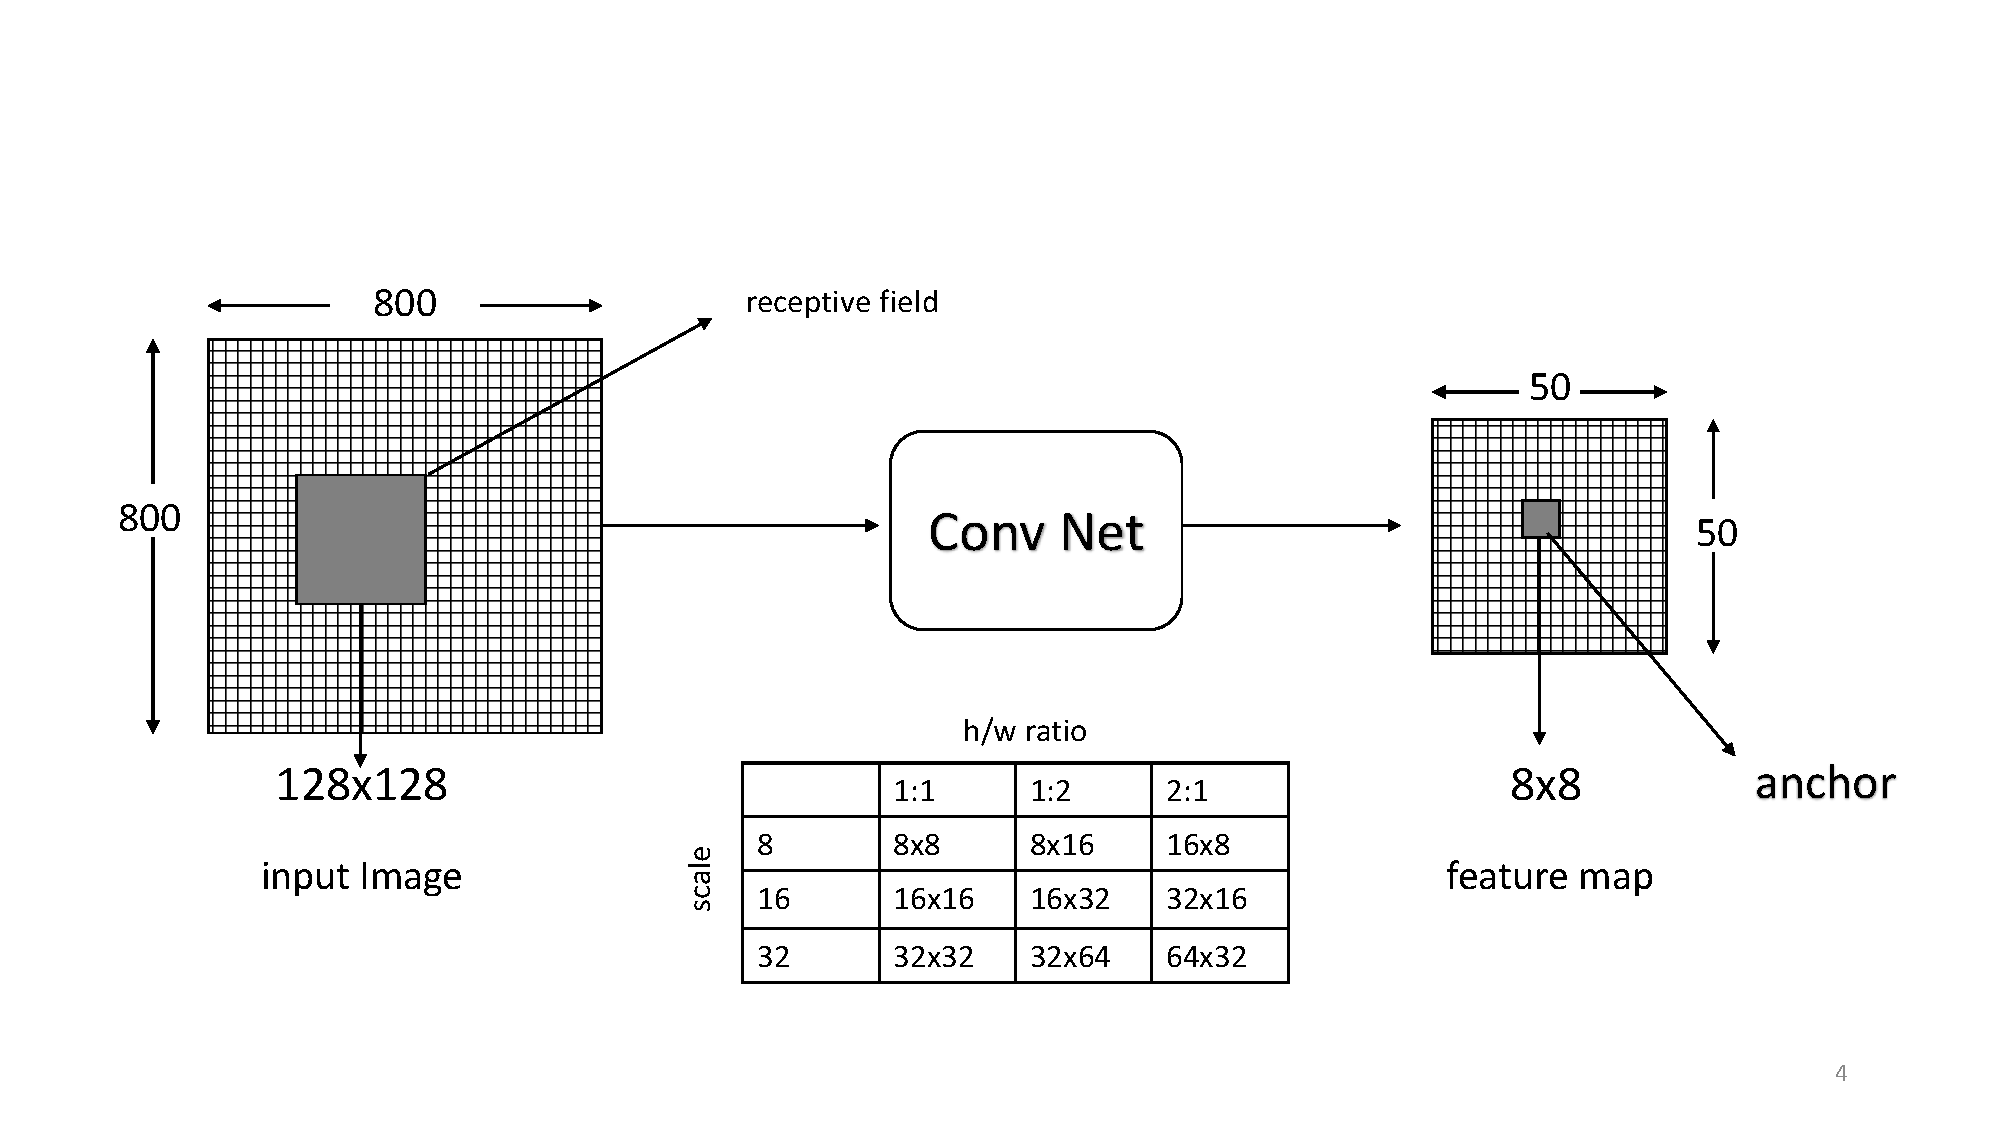
\includegraphics[width=\linewidth,trim={0 60 0 130},clip]{images/anchors}
    \caption[Anchor illustration]{Anchor illustration}
    \label{fig:anchors}
\end{figure}

\vspace{5pt}
\textit{b. Architecture of RPN}\\
Figure \ref{fig:RPN-architecture} shows the architecture of RPN sub-network. Input to this network are the features generated by the backbone network discussed in Section \ref{sec:feature-extraction}. These features are passed through a $3\times3$ ``same\footnote{$(h,w)$ of input and output feature map remains same by automatic padding}'' convolution layer. Faster-RCNN uses the 512 output feature depth for this layer. Output of this layer is fed to the bounding box regressor layer and objectness layer which predicts bounding box locations and objectness score simultaneously.
Both of these layers are modeled with $1\times1$ convolution. Bounding box regressor layer has $4k$ output depth where $k$ is the number of anchors and 4 follows from the fact that each proposal is defined by 4 scalar values. For similar reasons, objectness layer has $2k$ output features. Thus each anchor produces a proposal. All of these proposals are post-processed by the Non Maximum Suppression (NMS) algorithm. 


\begin{figure}
    \centering
    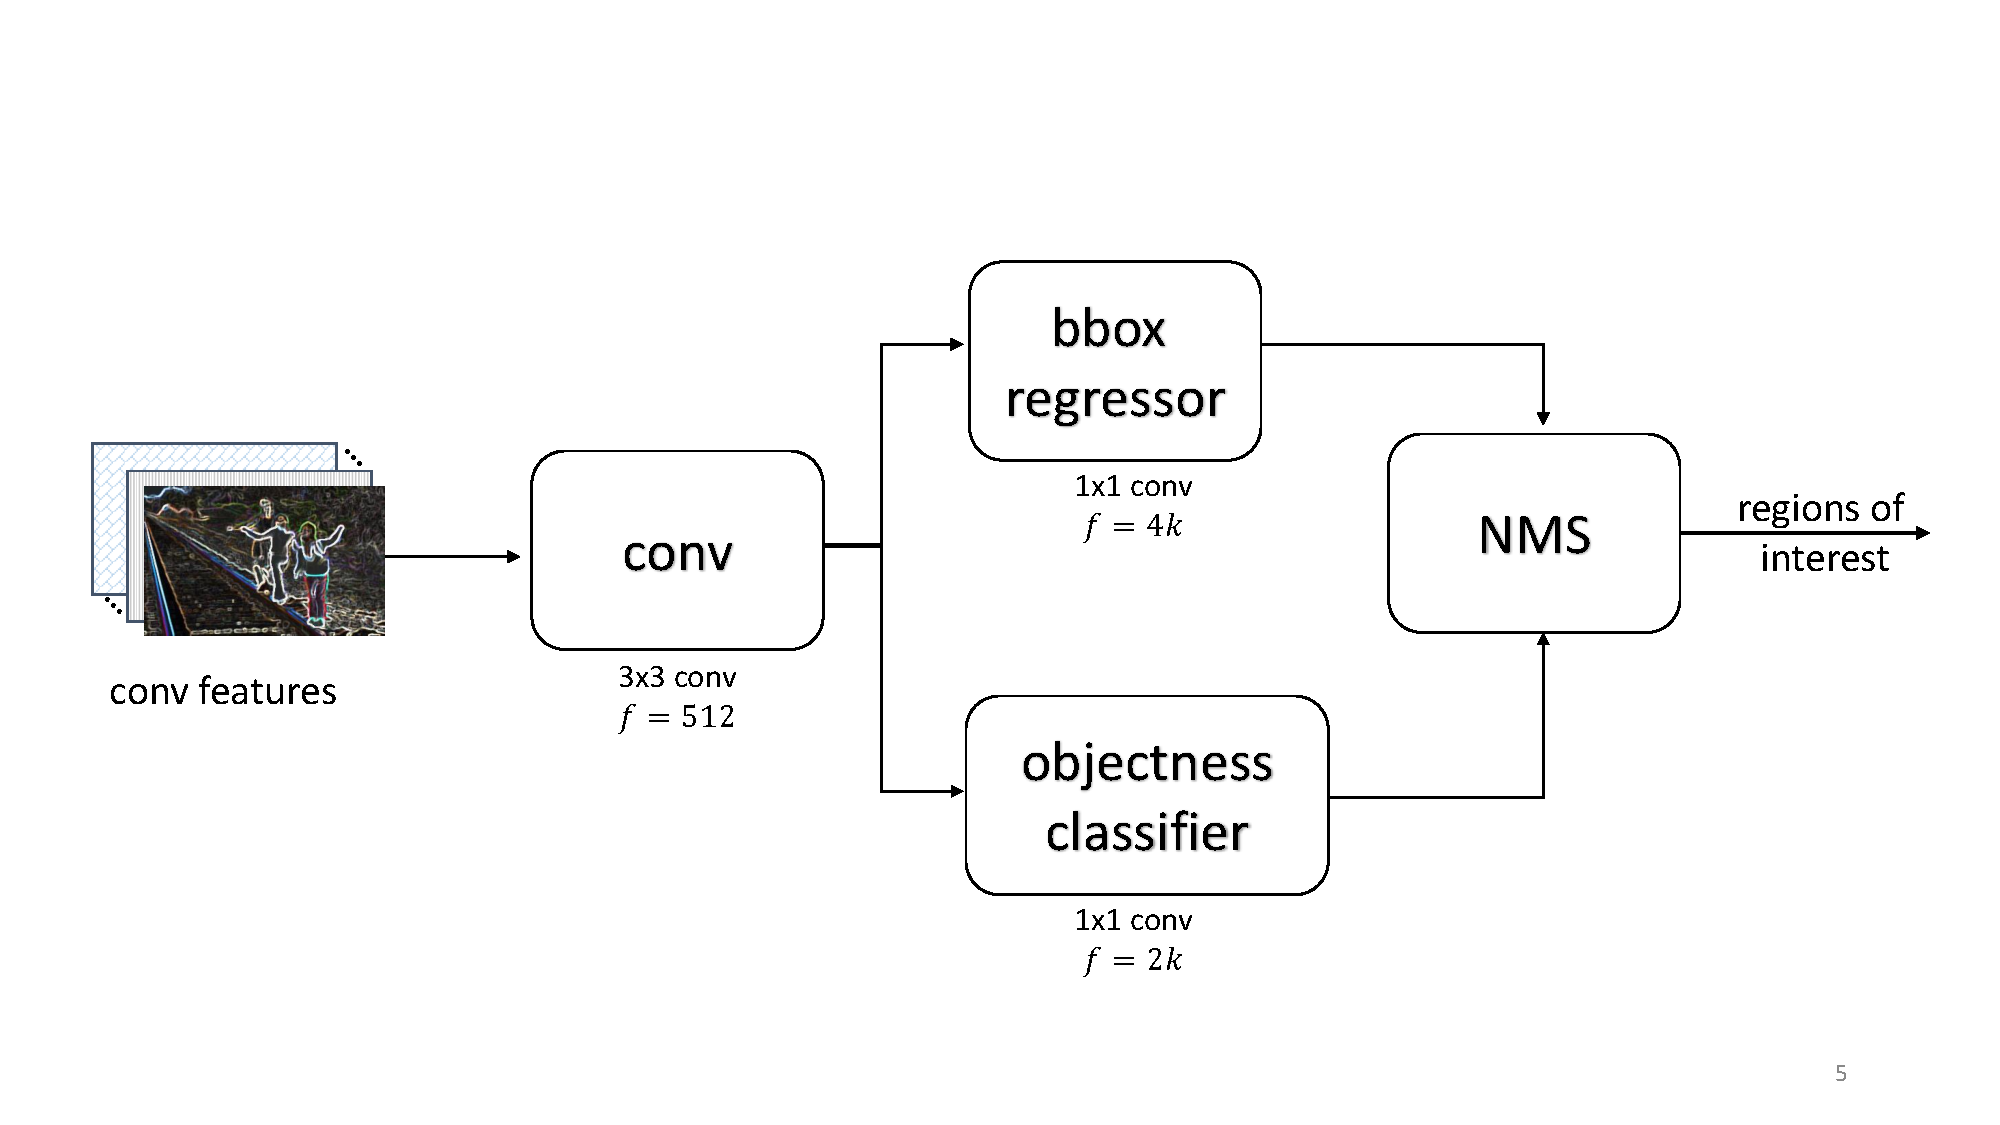
\includegraphics[width=\linewidth,trim={0 70 0 110},clip]{images/RPN-architecture}
    \caption[RPN architecture]{Region Proposal Network architecture}
    \label{fig:RPN-architecture}
\end{figure}


\vspace{5pt}
\subsubsection{Non maximum suppression (NMS)}
NMS is responsible for removing the duplicate predictions. Figure \ref{fig:nms} illustrates the goal of this process graphically. In order to suppress the duplicate proposal predictions with the less confidence, first step is to sort all the proposals in descending order. The first proposal is made  the reference proposal and pushed to ``keep'' list. Intersection over Union (IoU) of this reference proposal with all the remaining proposals is computed and the proposals which sufficiently overlap with the reference proposal ($IoU > 0.7$) are discarded. They are considered to be the duplicate of the reference proposal. In the next iteration, the first proposal in the list of undecided proposals is made reference proposal and the process of first iteration is repeated. Again this leads to removal of all the proposals considered to be duplicate of the reference proposal. The process continues until all the proposals are decided i.e. either kept or discarded. Output of this process is the list of ``kept'' proposals. 

\begin{figure}
    \centering
    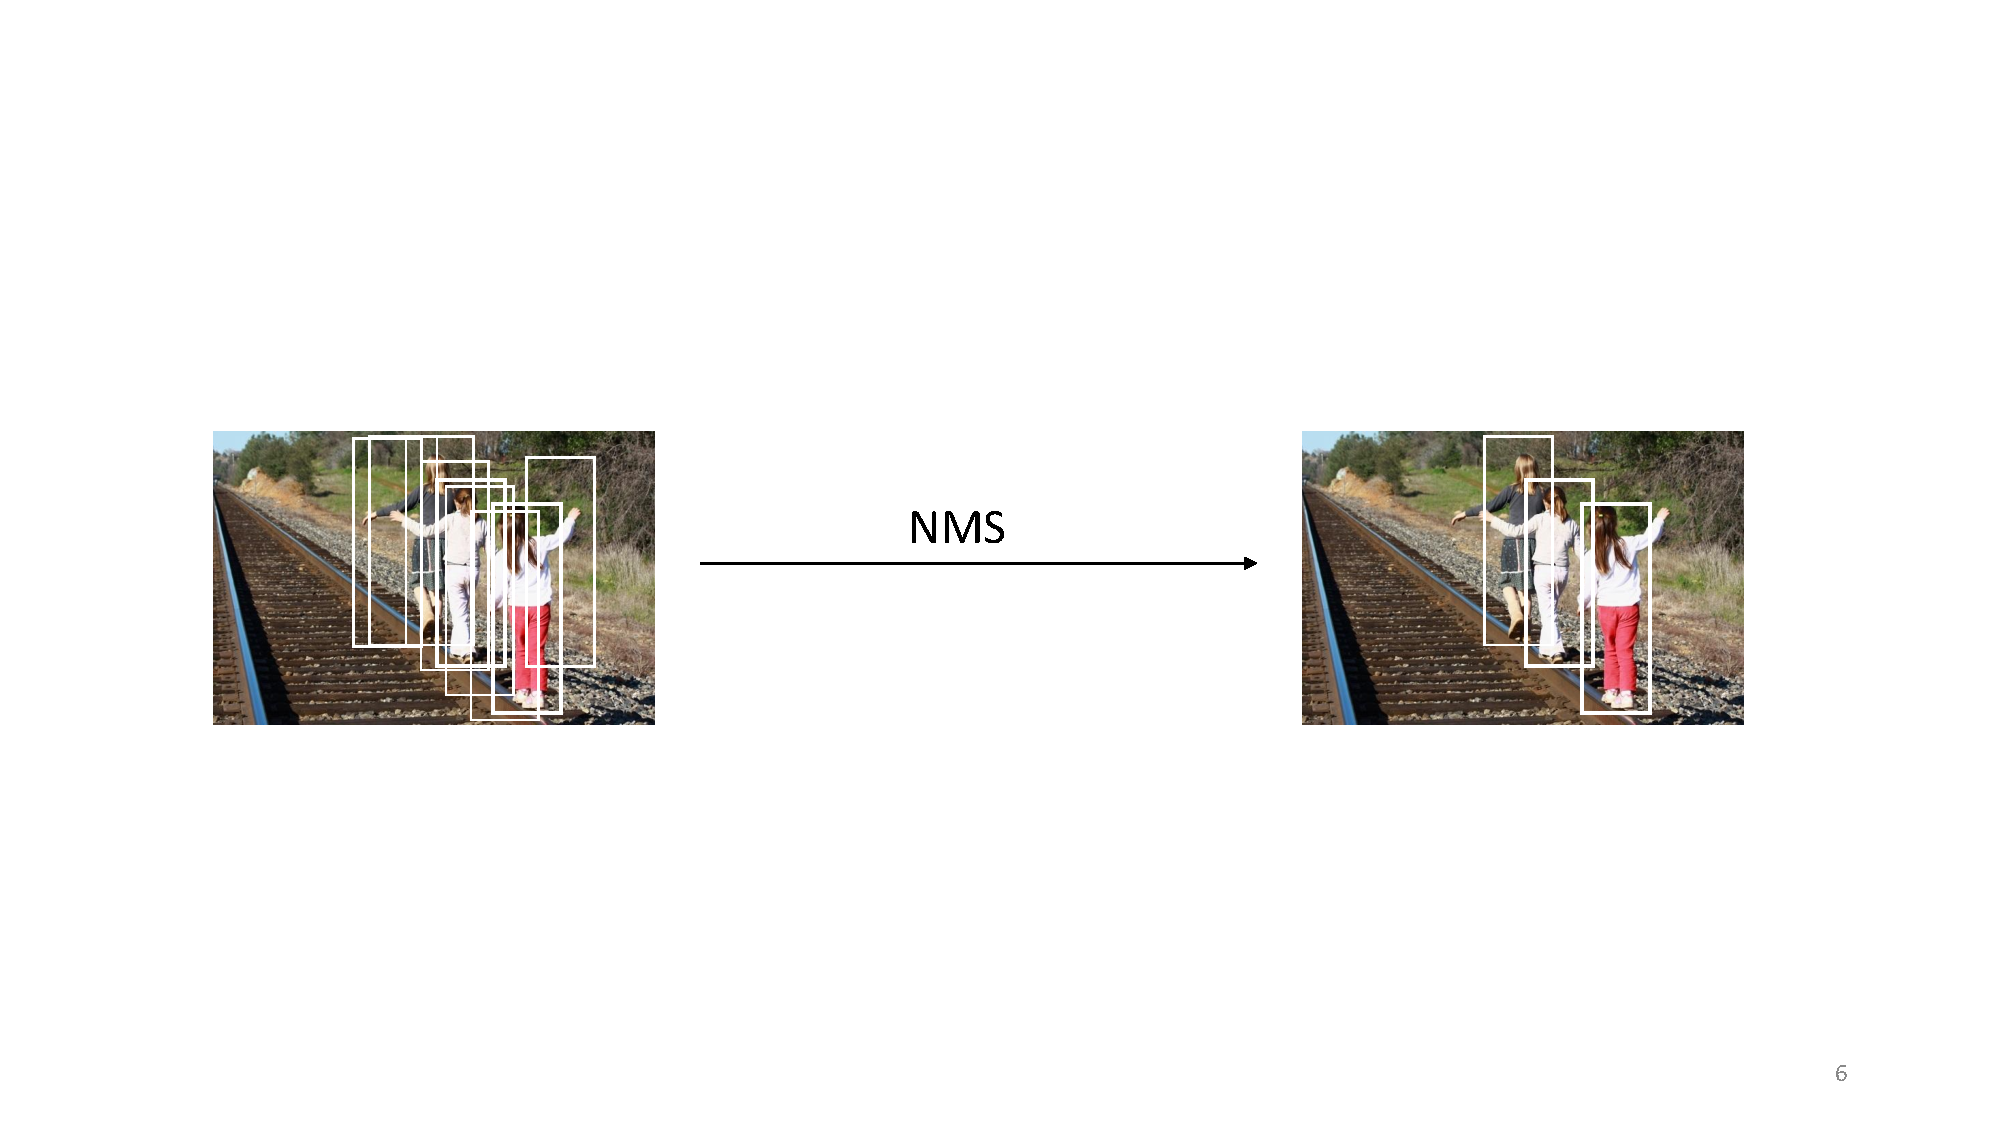
\includegraphics[width=\linewidth,trim={0 150 0 150},clip]{images/nms}
    \caption[Non Maximum Suppression (NMS)]{Non Maximum Suppression (NMS). Highly overlapping predictions with lesser confidence are suppressed.}
    \label{fig:nms}
\end{figure}

\vspace{5pt}
\subsubsection{Fast-RCNN head}
Once we have the proposals from RPN, we need to predict the corresponding objects' labels and locations. Faster-RCNN uses Fast-RCNN head\cite{ref_fastrcnn} for this purpose. Fast-RCNN head has two further sub-components. First one is the Region of Interest (RoI) pooling and second one is the classifier layer (Figure \ref{fig:faster-rcnn-pipeline}). Input to the Fast-RCNN head will be the feature map and the list of kept proposals; and output shall be improved bounding box locations of the corresponding proposals along with class labels. 

Different proposals have different feature map sizes. However, the classifier expects them to be of same size. RoI pooling is responsible for converting variable sized feature maps into fixed sized. The methodology used by Fast-RCNN in this case is quite simple. Suppose a feature map of size $8\times 8$ has to be converted to $2 \times 2$ size. Then, a grid of size $2 \times 2$ is placed on top of the feature map such that its boundaries align with the feature map. The maximum feature value from each grid cell is copied to corresponding cell in the output buffer. This converts a $8\times 8$ feature map to a size of $2 \times 2$.

Once RoI pooling has adjusted the size of feature map to fixed dimensions, the feature maps are ready to be fed to the classifier. The classifier takes in those features and passes them through two fully connected layers. The output of those two layers is fed to two separate fully connected layers responsible for predicting bounding boxes and object class labels. The bounding boxes and labels so predicted are the final output of Faster-RCNN. Figure \ref{fig:classifier} illustrates the architecture of classifier.

\begin{figure}
    \centering
    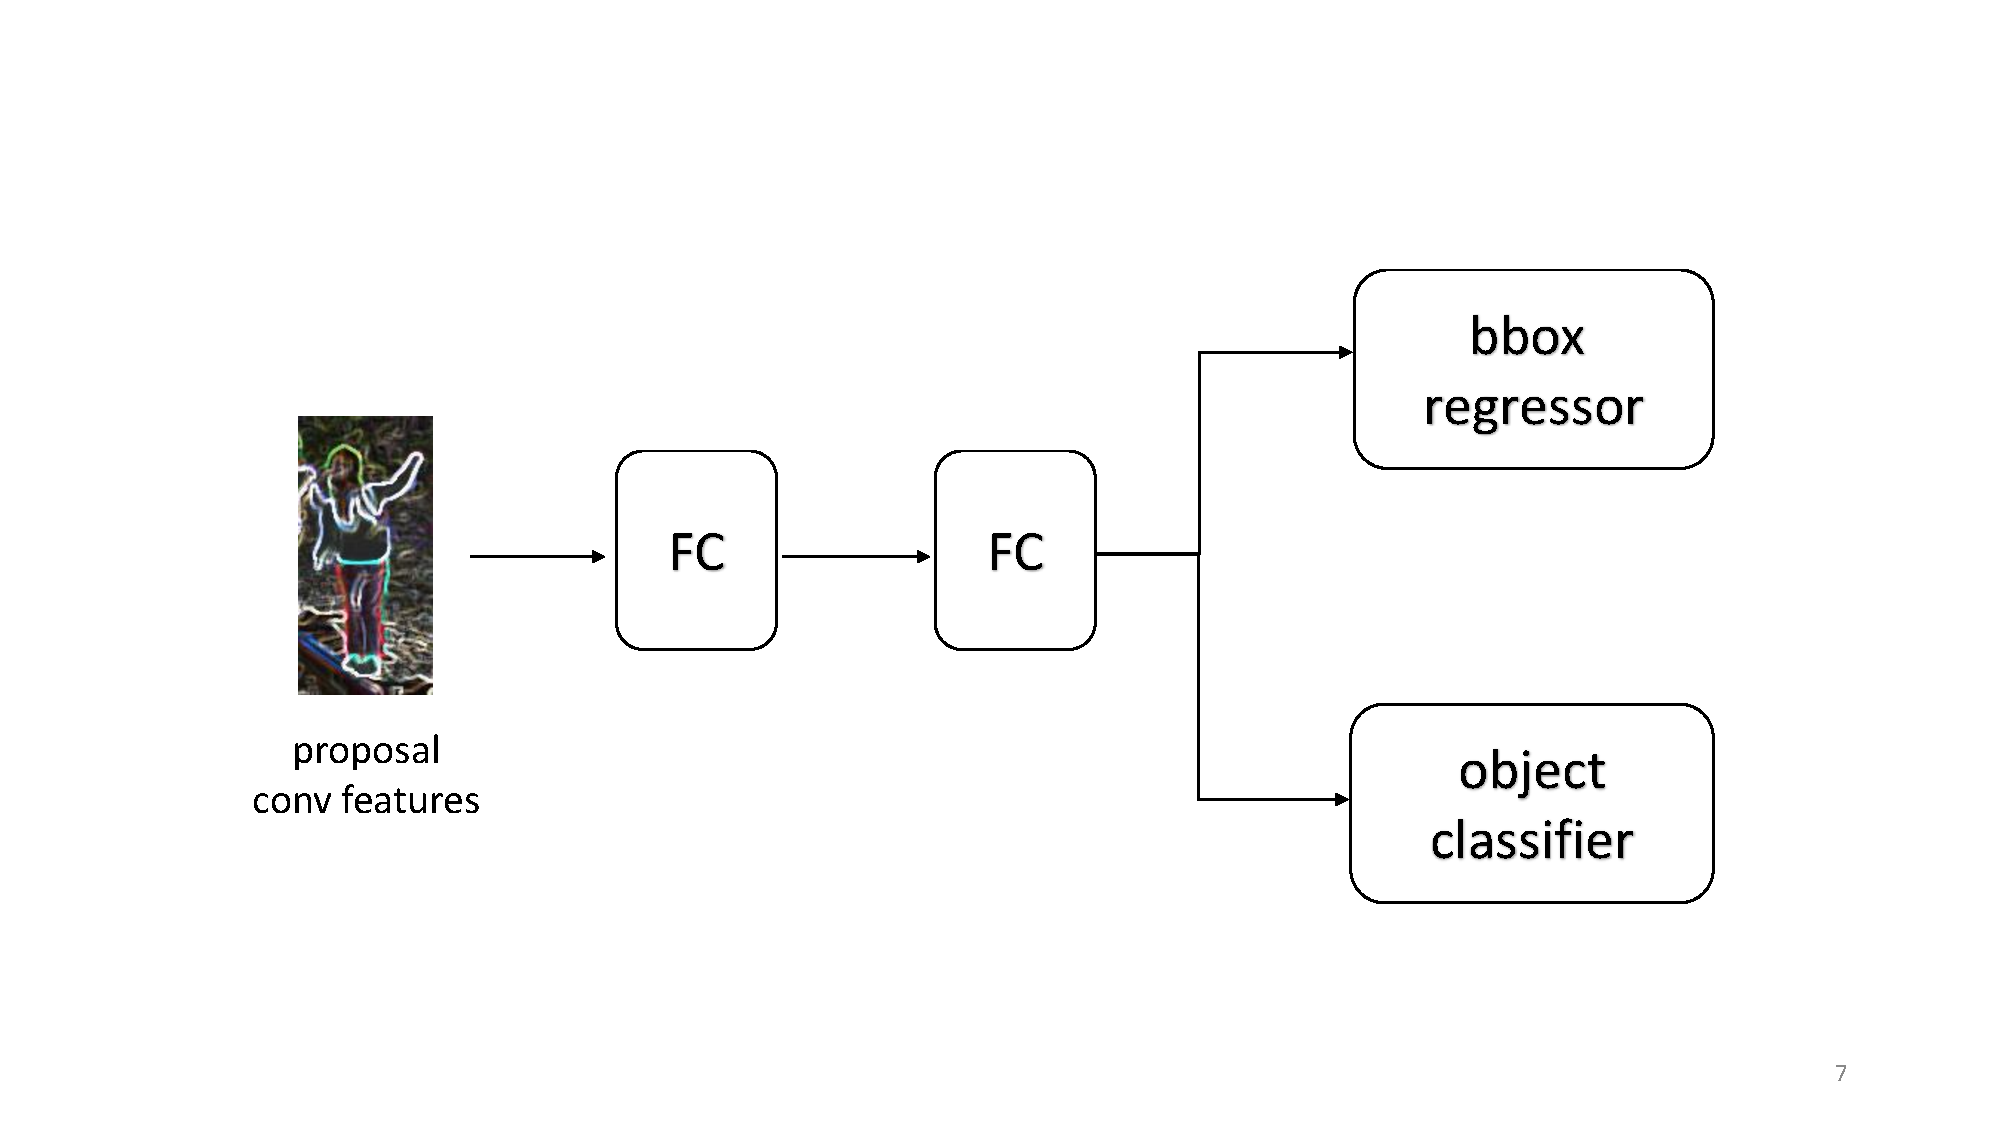
\includegraphics[width=\linewidth,trim={0 90 0 120},clip]{images/classifier}
    \caption{Fast-RCNN classifier}
    \label{fig:classifier}
\end{figure}

\subsubsection{Training loss}
While training the Faster-RCNN, we train two sub-networks: RPN and classifier. Both of these networks have two objectives: label classification and bounding box regression. Following two equations model the RPN and classifier loss. The first term corresponds to the label classification while the second term corresponds to the bounding box regression. 

$$Loss_{RPN}= \frac{1}{N_{cls}}\sum_i L_{cls}(\hat{p}_i,p_i) + \frac{\lambda_r}{N_{reg}}\sum_i p_i L_{reg}(\hat{t}_i,t_i)$$

\begin{small}
$$Loss_{cla} = \frac{1}{N_{cls}}\sum_i L_{cls}(\hat{q}_i,q_i) + \frac{\lambda_c}{N_{reg}}\sum_i [q_i > 0] L_{reg}(\hat{u}_i,u_i)$$
\end{small}
% where \\
% $\hat{p}_i=$ anchor label prediction \\
% $\hat{t}_i=$ anchor bounding box prediction \\
% $\hat{q}_i=$ RoI label prediction \\
% $\hat{u}_i=$ RoI bounding box prediction \\
% ${p}_i=$ anchor ground truth label \\
% ${t}_i=$ anchor ground truth bounding box  \\
% ${q}_i=$ RoI ground truth label  \\
% ${u}_i=$ RoI ground truth bounding box  \\
% $\lambda_r =$ RPN loss balance coef. \\
% $\lambda_c =$ classifier loss balance coef. \\
% $N_{cls}=$ mini-batch size \\
% $N_{reg}=$ total anchors
Table \ref{table:variable-list} defines the variables used in the above equations. Classification loss $L_{cls}$ is the standard log loss, and regression loss $L_{reg}$ is the smooth-$L_1$ loss as defined below. 

$$ L_{cls}(\hat{y},y) = -\sum_j y_jlog(\hat{y}_j) $$
$$ L_{reg}(\hat{b},b) = \sum_{j=1}^4 SL_1(\hat{b}_j - b_j) $$
$$SL_1(x) = \begin{cases}
0.5x^2, & \text{if } |x|<1 \\
x-0.5,  & \text{otherwise}
\end{cases}
$$
where input parameters to each function carry the standard meaning. The total loss of the network is the sum of RPN loss and classifier loss.
$$ Loss = Loss_{RPN} + Loss_{cla} $$

Apart from that notice the term $p_i$ in regression term of RPN loss. This makes sure that regression loss is activated only if proposal corresponds to an object, not to the background.  Thus bounding box predictions corresponding to background proposals do not contribute towards training. Further, the expression $[q_i>0]$ serves a similar job in the classifier loss. This again acts as a flag to add regression loss only corresponding to the actual objects and not the background. 

$\lambda_r$ and $\lambda_c$ act as the balancing parameters between label classification and bounding box regression. The authors of Faster-RCNN claim that $\lambda_r$ is redundant and Faster-RCNN remains insensitive to a large range of $\lambda_r$. 

\begin{table}
    \centering
\caption{Description of variables used in loss function}
\label{table:variable-list}
    \begin{tabular}{| l | l |} \hline
variable & description \\ \hline \hline
$\hat{p}_i$ & anchor label prediction \\ \hline 
$\hat{t}_i$ & anchor bounding box prediction \\ \hline 
$\hat{q}_i$ & RoI label prediction \\ \hline 
$\hat{u}_i$ & RoI bounding box prediction \\ \hline 
${p}_i$ & anchor ground truth label \\ \hline 
${t}_i$ & anchor ground truth bounding box \\ \hline 
${q}_i$ & RoI ground truth label \\ \hline 
${u}_i$ & RoI ground truth bounding box  \\ \hline 
$\lambda_r $ & RPN loss balance coef. \\ \hline 
$\lambda_c $ & classifier loss balance coef.  \\ \hline 
$N_{cls}$ & mini-batch size  \\ \hline 
$N_{reg}$ & total anchors \\ \hline 
    \end{tabular}
\end{table}{}